% Chapter 3

\chapter{Related Works} % Main chapter title

\label{Chapter2} % For referencing the chapter elsewhere, use \ref{Chapter1} 

\lhead{Chapter 2. \emph{Case Studies}} % This is for the header on each page - perhaps a shortened title

%----------------------------------------------------------------------------------------

Section \ref{staticEnergyMap} and section \ref{dynamicMap} provide an
overview of the existing instances of static energy maps and dynamic
energy maps. The static maps examples are arranged in the order of
increasing layers of information from heat mapping to energy potential
mapping of various energy sources and sinks. A summary of techniques
used to produce these Static and Dynamic Energy Map instances are
shown in \tref{tab:mapSummary}:

\begin{comment}
Section \ref{mapDesign} and \ref{stDataAnalysis} provides
some supporting evidences for certain design choices. Section
\ref{4dMap} provides some information on potential technologies for
further development. \grey{(?? are not written)}
\end{comment}

\begin{table}[h!]
  \centering
  \begin{tabular}{r|c|p{4cm}}
    \hline
Project Name           &Type   & Software \\
    \hline
    \hline
Calgary Map            &Static, Stand-alone &     ?    \\
    \hline
London Heat Map        &Static, web, interactive &ArcGIS WebApp\\
    \hline
National Heat Map      &Static, web, interactive &Google Map API \\
    \hline
Water Source Heat Map  &Static, web, interactive &Google Map API \\
    \hline
Dutch Heat Map         &Static, Stand-alone&     ?    \\
    \hline
Lowe Hill District Map &Dynamic, web, interactive&ArcScene, ArcMap,
                                                   GIS Cloud, excel  \\
    \hline
Energy Mapping to      &Dynamic, Stand-alone&QGIS      \\
Identify Opportunities & &          \\
for Future Network     & &          \\
    \hline
  \end{tabular}
  \caption{Map Technology Summary Table}
  \label{tab:mapSummary}
\end{table}

\section{Static Energy Map}\label{staticEnergyMap}
\subsection{UK Heat Map}
Under the goal of supplying 25\% of the total energy with
decentralized energy (DE) by the year 2025, the Decentralised Energy
Master Planning Program (DEMaP) was conducted between 2008 to 2010 to
``identify opportunities for district heating networks through heat
mapping and energy masterplanning''~\cite{londonHeatMap}. In this
study, the term DE only refers to ``combined heat and power systems
connected to district heating
networks''~\cite{decentralHeatMap2011}. 

London Heat Map is a publicly accessible interactive map developed as
part of the DEMaP project. It is completed for the London Boroughs in
2012. It can act as a starting point of Energy Master Plan for local
authorities, and can assist developers to make connections to existing
DE networks to meet policy requirements (London Plan DE
policy)~\cite{decentralHeatMap2011, londonHeatMap}. Point features of
high heating energy consumers and suppliers, existing and emerging
energy networks are depicted on the interactive map. High DE potential
regions (``focus area''~\cite{decentralHeatMap2011}) are identified
and depicted on the map to highlight the opportunities of utilizing
the heat supply in the community planning and development
(\fref{fig:londonHeat}). The ``live-database'' property of London Heat
Map allows new data of energy consumption be uploaded by users.

The criteria applied for identifying focus area include: 1) near to
existing or emerging DE network, 2) high heat demand density 3) anchor
load building, 4) diverse heating demand profile 5) has public
ownership with policy concerns to make connections to the DE
network~\cite{decentralHeatMap2011}. The physical constraint are also
considered in finalizing the high DE potential regions.
\begin{figure}[h!]
  \centering
  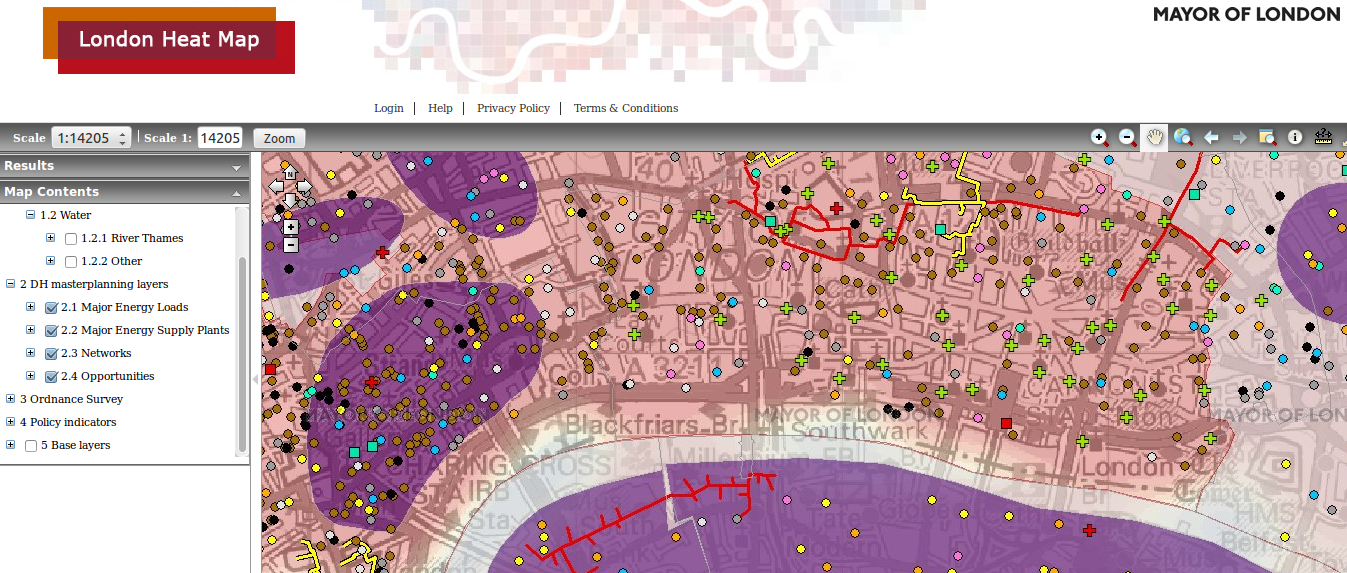
\includegraphics[width=0.7\linewidth]{londonHeat.png}
  \caption[London Heat Map]{London Heat Map~\cite{londonHeatMapMap}}
  \label{fig:londonHeat}
\end{figure}

National Heat Map (\fref{fig:nhm}) is another UK energy mapping
project that focuses more on the industry
side~\cite{decentralHeatMap2011}. It is a ``high resolution
web-based'' heating energy interactive map, developed by the
Department of Energy and Climate Change (DECC). It aims at ``support
planning and deployment of local low-carbon energy projects in
England''~\cite{heatMap2015}. Power plant developers can use this map
to consider the feasibility for a CHP plant under policy
requirements~\cite{decentralHeatMap2011}. Heating demand density
($kWh/m^2$) of four major building sectors: public buildings,
commercial buildings, industry buildings and residential buildings,
together with the total demand is plotted on the map as a 2D raster
image with a discrete color scheme from blue to red representing low
to high heating demand. Heat source of CHP stations and thermal power
stations are plotted as point features in the map. Address level heat
demand data in csv format is also available for local authorities upon
request~\cite{heatMapLocal2012}.

\begin{figure}[h!]
  \centering
  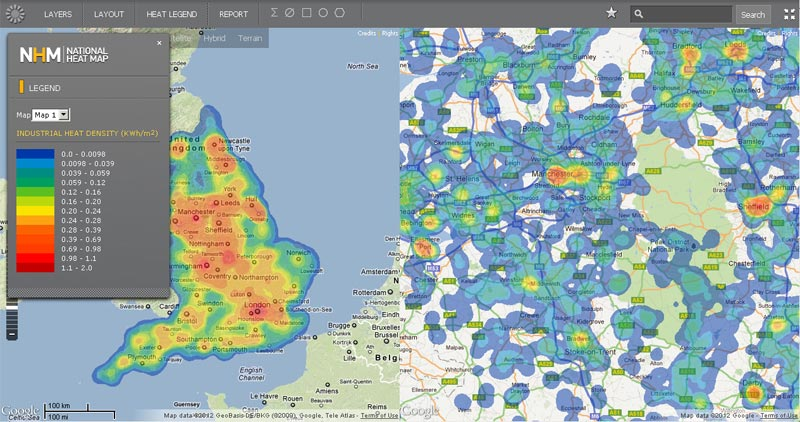
\includegraphics[width=0.5\linewidth]{nhm.jpeg}
  \caption[National Heat Map]{National Heat Map~\cite{heatMap2012}}
  \label{fig:nhm}
\end{figure}

The ``Water Source Heat Map'' (\fref{fig:waterMap}) is an added layer
group to the existing National Heat Map with information about the the
heat potential of the 4041 waterways in England. Heat potential of
waterways are represented in temperature, surface area, flow rate and
heat capacity ($kJ/m^3$ for coastal and estuary, $kW$ for canal, river
and settlement). It aims at supporting the plan of water-based thermal
system as water-based heat pump~\cite{waterHeatMap}. The map revealed
the large thermal capacity of water bodies that could serve over one
million buildings in the UK~\cite{waterHeatMap}.

\begin{figure}[h!]
  \centering
  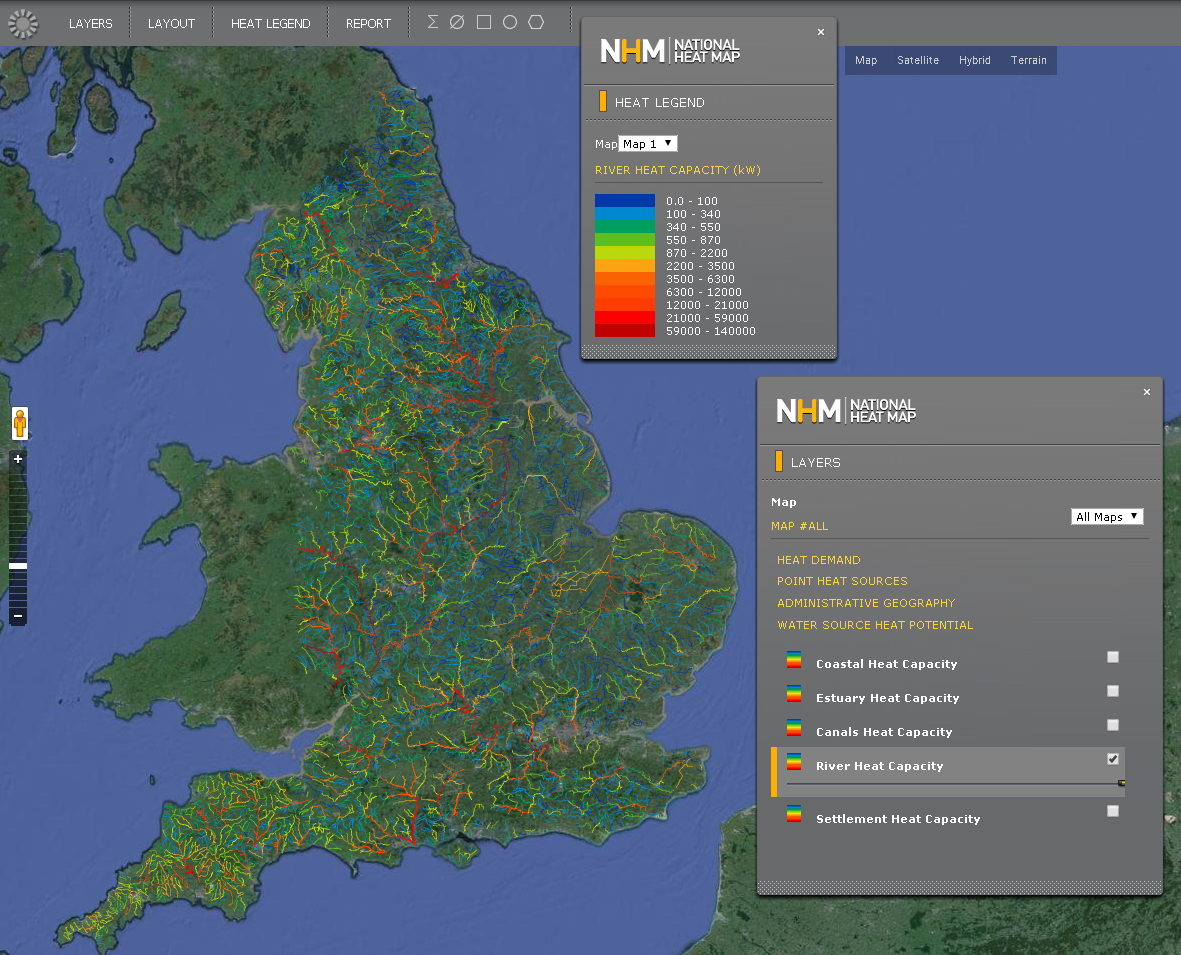
\includegraphics[width=0.5\linewidth]{waterMap.png}
  \caption[Water Heat Map]{Water Source Heat Map~\cite{waterHeatMap}}
  \label{fig:waterMap}
\end{figure}


\subsection{Calgary Energy Map}
One of the early instances of Static Energy Mapping is the Energy
Mapping Study of City of Calgary in 2008, carried out by Canadian
Urban Institute. It aims at providing insights to achieve the goal of
reducing 50\% of Green House Gas (GHG) emissions by
2050~\cite{aacip2009}. It depicts 1) how building design strategies
and land use planning can influence the city level energy use
intensity 2) the availability of alternative energy sources and the
opportunities to combine building level sustainable design technology
with the community level energy system design.

Calgary energy map first compares energy use intensity (the annual
total demand for thermal energy of space heating cooling, hot water
and electricity per unit area~\cite{aacip2009}) in GJ/ha between two
development cases: ``business as usual'' case and ``ultra-high
efficiency'' case (\fref{fig:calgaryCmp}). The comparison demonstrated
a 34\% reduction in energy use intensity from the former to the
latter~\cite{aacip2009}.

\begin{figure}[h!]
  \centering
  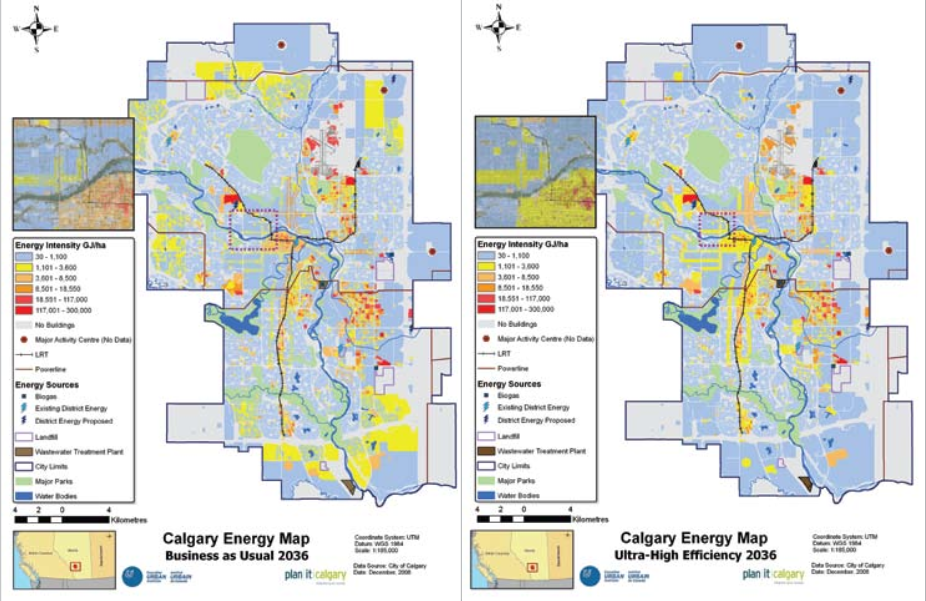
\includegraphics[width=0.6\linewidth]{calgaryCmp.png}
  \caption[Calgary Energy Demand Map]{Calgary Energy Map (Business as Usual, Ultra-High
    Efficiency)~\cite{aacip2009}}
  \label{fig:calgaryCmp}
\end{figure}

It also shows alternative energy sources of district energy, solar hot
water, solar air, energy sharing and PV installation on the map
(\fref{fig:calgaryAlter}). By overlaying the alternative technology
map and the ``ultra-high efficiency'' map, it highlights the
opportunities of using alternative renewable energy sources and
district energy system to further improve the energy performance of
high energy demand areas after high performance building design was
applied~\cite{aacip2009}.

\begin{figure}[h!]
  \centering
  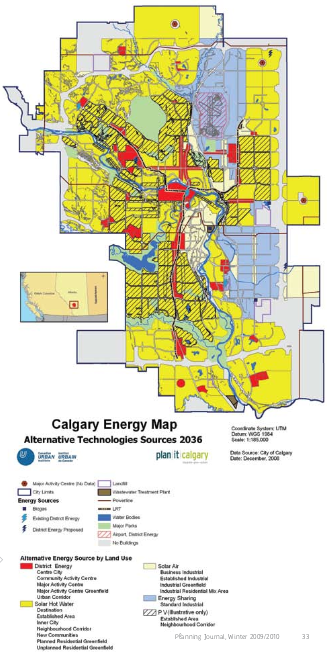
\includegraphics[width=0.3\linewidth]{calgaryAlter.png}
  \caption{Calgary Energy Map Alternative Energy Source~\cite{aacip2009}}
  \label{fig:calgaryAlter}
\end{figure}

\subsection{Energy Potential Mapping}
Dobbelsteen et al. described a framework of Energy Potential Mapping
(EPM) that aggregates information of energy supply, demand and
infrastructure on the same map with demand and supply represented in
the same unit of GJ or GJ/ha~\cite{Dobbelsteen2013}.

In 2010, a ``Heat Mapping'' study under the framework of EPM was
launched by TU Delft aiming at visualizing heat demand and supply and
infrastructure with the same unit that facilitates easy comparison and
facilitates the matching of supply and
demand~\cite{Dobbelsteen2013}. The map is presented with aggregated
supply and demand in a 3D Heat Map. The absolute quantity of each type
of demand and supply is represented with extruded height in the 3D
map. Demand is represented with a transparent 3D feature, and each
supply source is represented with solid 3D feature in a different
color~\cite{Dobbelsteen2013}.

\begin{figure}[htbp]
  \centering
  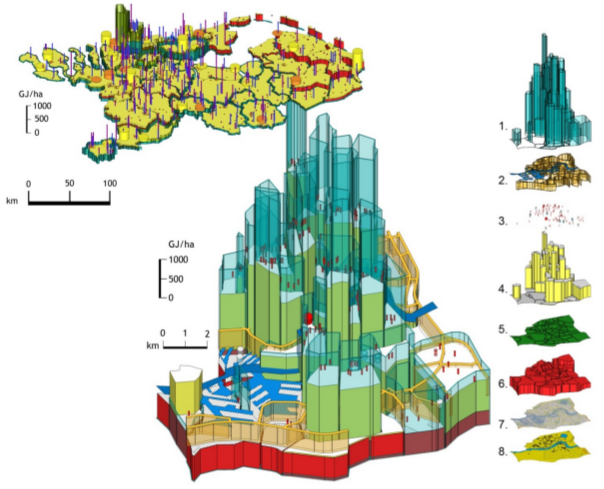
\includegraphics[width=0.7\linewidth]{heatmapNL.png}
  \caption[Rotterdam Heat Map]{Heat Mapping of Netherlands and
    Rotterdam~\cite{Dobbelsteen2013}}
  \label{fig:heatmapNL}
\end{figure}

\section{Dynamic Energy Map}\label{dynamicMap}
Per definition of Dynamic Energy Map in the introduction, there are
not instances that fully realized all the desired functions yet. In
this section, we will discuss some valuable attempts towards realizing
and exploring the power of dynamic energy mapping.

\subsection{Lower Hill District Dynamic Mapping Project}
In 2011 to 2012, the Dynamic Energy Map of the Lower Hill District,
Pittsburgh, PA was created. It is designed to conduct feasibility
analysis and comparison of alternative energy supply techniques of a
district energy system~\cite{baird2014, Ramesh2013}. A geo-data base
was created with ArcMap, ArcScene and Sketchup. In the database, each
building, represented as a 3D feature, contains attributes of its
building name, annual energy consumption, energy use intensity (EUI),
and annual and monthly peak demand. The map is online accessible via
GIS Cloud (\fref{fig:mellonArenaGIS}).

\begin{figure}[h!]
  \centering
  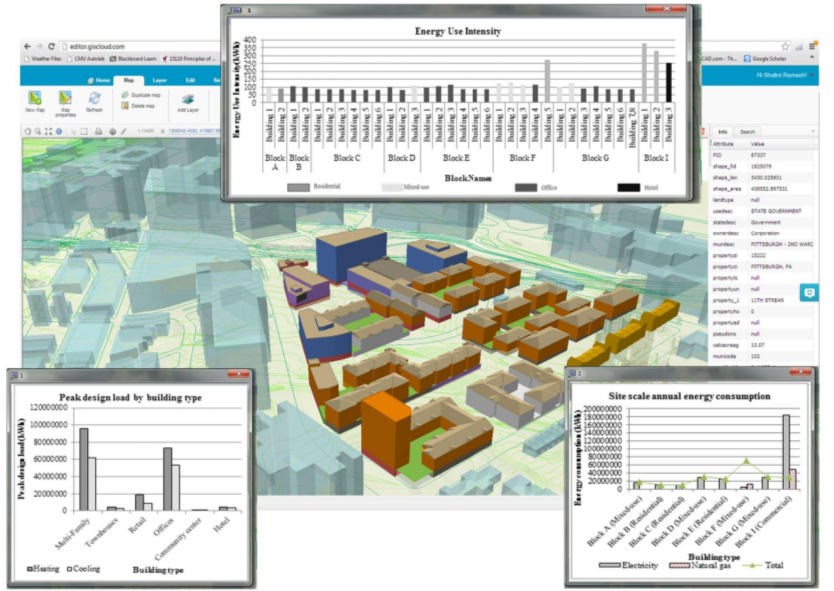
\includegraphics[width=0.7\linewidth]{mellonArenaGIS.png}
  \caption[Lower Hill District 3D GIS Map]{Online Accessible GIS-database with GIS
    Cloud~\cite{baird2014, Ramesh2013}}
  \label{fig:mellonArenaGIS}
\end{figure}

The feasibility analysis and temporal data display are separated from
the geo-database and is performed in a excel screening tool. The tool
takes input of energy cost rate, building type and size, development
phase and central plant types and feature and produces a feasibility
analysis and related temporal graphs (\fref{fig:3dexcel}) of annual
hourly energy consumption for each building type and the aggregated
demand of natural gas, cooling use electricity and total electricity.

\begin{figure}[h!]
  \centering
  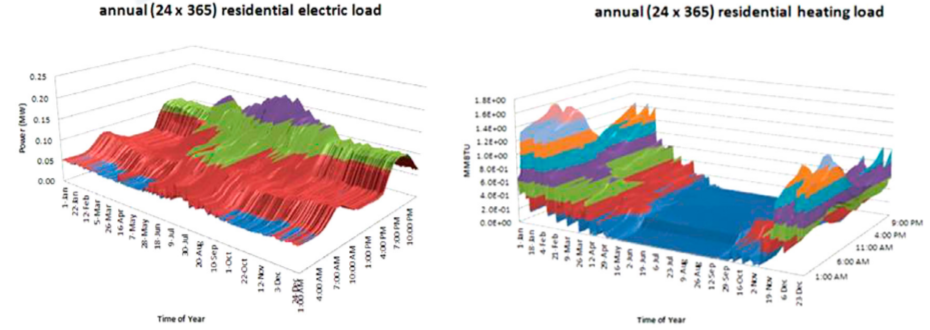
\includegraphics[width=0.7\linewidth]{3dexcel.png}
  \caption[Heating/Electricity Residential]{Heating Load and
    Electricity Load for Residencial Building~\cite{baird2014}}
  \label{fig:3dexcel}
\end{figure}

\subsection{Energy Mapping to Identify Opportunities for Future
  Networks Project}
Another instance of energy demand dynamic map with high spatial
resolution was found in the project ``Energy Mapping to Identify
Opportunities for Future Networks''~\cite{Diaz2013}. The aim of the
project is to ``analyze the spatial and temporal distribution of
energy consumption'' and support decision making and design of energy
network: more specifically, to identifiy opportunities of District
Heating, CHP plant development and Building Design
Improvement~\cite{Diaz2013}.

Energy Demand Maps of three different resolutions were created using
QGIS: campus level, community level and city level. Energy data was
retrieved from both metered data (used in campus level map) and HEM
simulation (used in community and city level map). HEM is a tool for
``mapping the possiblemapping the possible carbon and energy
performance of a dwelling. It has pre-simulated results embedded as a
data table in the tool and applies the appropriate system and context
calculations to provide instant energy, carbon and cost results''~\cite{HEMesru2015}.

For the campus level map, the heat demand density (heat demand over
conditioned area) were depicted to identify ``outliers'': the
buildings with high heat demand~\cite{Diaz2013campus}. These outliers
were potential buildings need to be improved in building insulation
level or HVAC system efficiency. They claim a spatial map is
sufficient for this outlier identification process
(\fref{fig:heatGlasgow}). They also created a temporal spatial map of
monthly heat consumption that is in the form of both small multiples
(\fref{fig:seqheatGlasgow}) and non-interactive animated map
(\fref{fig:animeheatGlasgow}). With the dynamic map, they identified
two campus buildings with high heat demand through the whole year
(anchor load building) and concluded that the two buildings could
connect to a district heating system. They also created two animated
maps with electricity and natural gas. By comparing these two animated
maps, consistent high consumers for electricity and gas were
identified as potential candidate building for a micro-CHP
system~\cite{microCHP}.

\begin{figure}[h!]
  \centering
  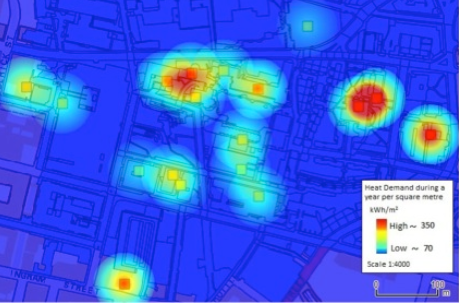
\includegraphics[width=0.5\linewidth]{heatGlasgow.png}
  \caption[Heat Demand Density]{Campus Level Heat Demand Density Map~\cite{Diaz2013campus}}
  \label{fig:heatGlasgow}
\end{figure}

\begin{figure}[h!]
  \centering
  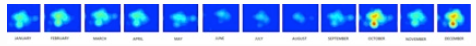
\includegraphics[width=0.5\linewidth]{seqheatGlasgow.png}
  \caption[Monthly Heat Demand (Small Multiple)]{Campus Level Monthly Heat Demand Map in Small Multiples\cite{Diaz2013campus}}
  \label{fig:seqheatGlasgow}
\end{figure}

\begin{figure}[h!]
  \centering
  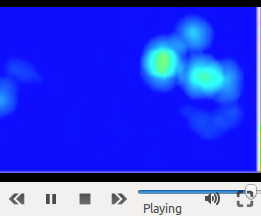
\includegraphics[width=0.3\linewidth]{animeheatGlasgow.png}
  \caption[Campus Animated Map]{Campus Level Monthly Heat Demand Map in Animation\cite{Diaz2013campus}}
  \label{fig:animeheatGlasgow}
\end{figure}

The community level spatial and temporal GIS analysis undertook a
similar process as the campus level except for the energy data is
retrieved from HEM simulation. By comparing the four different
building types: ``Traditional Build, New Build, Council Estate, High
Rise Flat'', they identified the consistent high gas and electricity
demand of High Rise Flat buildings. They also discovered that the
improvement of building design could adjust the heat to power ratio
(HTP) and could make applying CHP option feasible~\cite{Diaz2013com}.

City level map does not contain temporal mapping analysis and is left
out from the case study~\cite{Diaz2013city}.